\section{Machine Learning}

\paragraph{} Commençons par nous arrêter un instant sur le terme de \emph{Machine Learning}. En français,
cela pourrait se traduire par \emph{L'apprentissage de la machine}. Mais quel apprentissage ? N'est-ce pas
le rôle de l'Homme, comme nous l'avons soutenu jusqu'ici, d'apprendre à la machine ? Nous verrons que dans
le cas du Machine Learning, le concepteur ne fait que \emph{construire un système}, et lui donner
\emph{les clés} pour parvenir à la résolution d'un \emph{problème complexe}. On remarque ici l'importance
de \emph{cibler} un domaine: lorsque nous parlons de ML, nous ne prétendons pas créer un système à l'image
humaine, qui serait capable d'avoir une faculté d'apprentissage \emph{globale}, quel que soit le support. 

\paragraph{} Justement, n'est-ce pas là une réelle différence entre l'apprentissage humain et celui de la machine ?
Lorsque l'Homme apprend, c'est par \emph{l'expérience}. Il fait l'expérience de son environnement et la
conséquence de l'action lui permet d'être \emph{mieux préparé} à la prochaine expérience. Mais c'est en fait un
comportement similaire qui est utilisé en Machine Learning : un agent est entraîné à partir d'un certain nombre
d'entrées, dont il tire une sortie. Ce résultat est comparé à celui qui était attendu, puis la machine est
\emph{reparamétrée}, de sorte à ce qu'une prochaine expérience similaire aboutisse à un résultat plus proche 
de celui escompté. Ce processus de reconfiguration par l'apprentissage intervient notamment au niveau du cerveau
chez l'Homme, ce qui est concrétisé en ML par l'utilisation de Réseaux Neuronaux ou Neural Networks (NN), dont
nous détaillerons l'utilisation par la suite. Ce qu'il faut retenir de la différence entre la méthode d'apprentissage
d'un Homme et d'une machine, c'est la capacité d'adaptation du tissu neuronal de l'Homme à une variété de situations
et de problèmes que la machine n'est pas capable d'appréhender seule.

\paragraph{Cerveau humain et Ordinateur}

\paragraph{} Afin de comprendre ces différences entre les capacités de l'Homme et de la machine, il nous faut nous
intéresser un instant à leur composition et à leur mode de fonctionnement. Rappelons en premier lieu qu'une machine
fonctionne sur un \emph{système binaire}, qu'elle est la seule à pouvoir comprendre. L'Homme de son côté réfléchit
par une infinité \emph{d'associations de sensations}, qui partent de son expérience sensorielle par les 5 sens : vue,
toucher, odorat, ouïe, goût. En ce sens la \emph{réflexion} est le propre de l'Homme, car il est seul à pouvoir 
apprendre par la projection de son expérience. \cite{Brain1}

\paragraph{} De plus, le cerveau humain possède une centaine de milliards de neurones, eux-mêmes connectés à plus de 10.000
de leurs voisins. Cette structure gigantesque n'est pas encore égalée par l'ordinateur, dont le nombre de cellules est de
l'ordre de 5 milliards, et sont contigües en mémoire. On remarquera néanmoins que l'information y circule
beaucoup plus rapidement que dans le cerveau, où les impulsions synaptiques atteignent 6 à 10 m/s. Enfin on remarquera que la
nature des mémoires est totalement différente : là où l'ordinateur est capable de \emph{stocker de l'information}, et est donc
capable de restituer une information de manière \emph{infaillible}, l'Homme doit compter sur les mémoires à court et long termes,
ainsi que sur ses registres sensoriels - ce qu'il connait de \emph{l'expérience}. \cite{Brain0}

\begin{figure}[h]
    \centering
    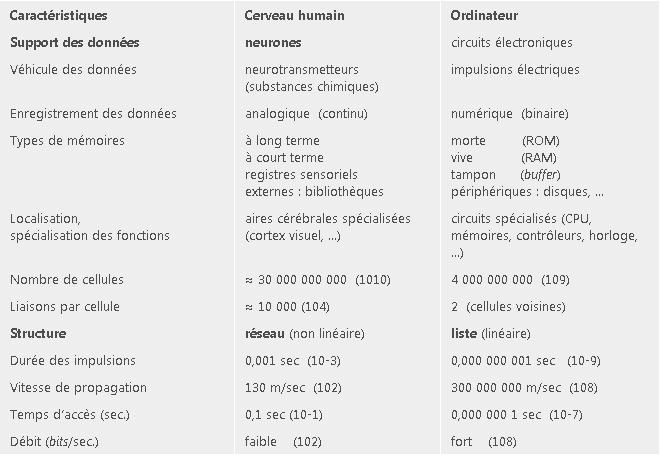
\includegraphics[width=350px]{chapters/03/images/cerveau-robot.jpg}
    \caption{\label{comparatif} \emph{Comparaison entre cerveau humain et ordinateur}, \cite{Brain1}}
\end{figure}

\paragraph{Résoudre des problèmes complexes}

\paragraph{} Pour mettre en avant la valeur ajoutée du Machine Learning, nous allons nous intéresser à l'exemple
du possesseur du chat appellé Ada \cite{MachineLearning0}. Il tente de poser la question suivante : qu'est-ce qu'Ada essaie de dire
à son maître lorsqu'elle ronronne quelques instants après avoir fait tomber la télécommande de la table basse ? Cela ne semble
pas avoir de réponse absolue en premier lieu, car il n'est pas possible de \emph{parler la langue d'Ada}. De fait, nous cherchons
donc une réponse \emph{appropriée}, c'est-à-dire au plus proche des attentes qu'avait eu
Ada auparavant, quand \emph{elle avait ronronné de la même manière}, ou \emph{dans un contexte similaire}. Une multitude de réponses
possibles s'ouvrent alors à nous : elle à peut-être faim, ou encore elle cherche de l'attention, ou bien elle n'aime pas les
télécommandes, ou elle aime simplement faire tomber des objets.. 

\paragraph{} Néanmoins, les ordinateurs font d'ores et déjà un nombre incalculable de choses que nous ne serions pas capables de faire
par nous-même comme la navigation, le calcul, le monitoring... serait-il donc possible que l'on construise un logiciel qui résolve le problème
d'Ada pour nous ? Cette question est fondamentale car elle nous demande de savoir si un ordinateur est capable d'apprendre à résoudre un
problème \emph{quelconque et indéterminé}. Si un logiciel peut comprendre Ada à partir de son observation, alors nous en déduisons qu'il devrait
être possible de lui donner n'importe quel système à observer afin qu'il puisse répondre à ses attentes.   

\paragraph{L'approche \emph{classique}} Afin d'écrire le logiciel qui répondrait au problème d'interprétation d'Ada, un développeur commun,
non initié au ML, devrait partir d'un ensemble de règles, parfaitement détaillées. Cela devrait reprendre tous les sons possibles émis par Ada,
les interprétations de ses comportements, de ses gestes, en fonction éventuellement du lieu, de la période... Tout cela afin de parvenir au 
\emph{message} qu'Ada est actuellement en train de transmettre. En somme, il faut arriver à figurer parfaitement, sous la forme de règles,
la représentation d'un problème particulier pour aboutir à la solution correcte. C'est-à-dire que le développeur devrait \emph{comprendre parfaitement}
Ada afin que l'ordinateur puisse atteindre la même compréhension, or nous réalisons bien que c'est impossible.

\paragraph{} Ce qu'il faut comprendre ici, c'est simplement que l'humain est \emph{faillible}. Il est toujours \emph{possible} qu'il se trompe
ou qu'il n'ait pas considéré les variables \emph{dans leur ensemble}. Nous pensons que ce n'est pas un mal en soi, et c'est bien le fait d'avoir accepté cette
faiblesse de l'humain par rapport à la machine qui lui a permis de remplacer l'un par l'autre dans des domaines où l'erreur n'est pas possible.
Il nous est impossible aujourd'hui d'imaginer la gestion des transports sans informatique, la santé sans matériel haute technologie afin de
permettre des analyses poussées, ou encore la finance sans tout le support des machines qui permettent notamment \emph{l'existence des marchés}. 

\paragraph{Une solution: le Machine Learning} Là où l'humain ne peut pas concevoir la complexité liée à la compréhension d'Ada, il semblerait que les
ordinateurs puissent quant à eux approcher une solution exploitable. D'ordinaire, afin de résoudre des problèmes, les ordinateurs utilisent des \emph{affectations}
(\emph{mapping}) de questions ou problèmes (en entrée) à des réponses ou solutions (en sortie). Tout le principe réside dans les étapes à respecter lors de
cette affectation, et nous avons pu voir qu'un développeur n'a pas toujours la réponse à cette question. De fait, pourquoi ne pas demander à une 
machine de se rendre compte \emph{elle-même} de la meilleure manière de réaliser cette affectation ? \cite{MachineLearning0} C'est exactement le propos du Machine
Learning. Il s'agit en général de renseigner \emph{d'immenses quantités} de données du problème afin qu'il adopte l'algorithme qui répond le mieux à
comment configurer ce \emph{mapping}. Cela est rendu possible, comme nous l'avons vu précédemment dans la section sur \emph{le cerveau et l'ordinateur},
par l'immense faculté de calcul \emph{infatigable} et \emph{infaillible} de la machine.

\paragraph{Sélectionner les données}\label{select_data_ml} Lorsque nous avons abordé le sujet de la collecte des données plus tôt, nous avons rapidement constaté la 
multiplication \emph{exponentielle} des données disponibles pour \emph{nourrir} de nouveaux logiciels d'apprentissage. Leur nombre n'est pas
uniquement un avantage car il augmente les chances qu'il y ait des données \emph{inutiles à notre problème}. C'est pourquoi il faut s'appliquer
d'une part à tenter de fournir des jeux de données \emph{restreints ou contrôlés} à nos machines, et à toujours faire attention d'y supprimer les
éventuelles données inutiles. Si vous souhaitez répondre au problème d'Ada, alors vous pouvez supprimer de vos données tout ce qui ne correspond
sous aucun aspect au domaine : finance, médecine, informatique.. Ces données sont une \emph{mauvaise herbe} et risquent de \emph{ralentir} ou de
\emph{compromettre} l'apprentissage de la machine. 

\paragraph{Plusieurs formes de Machine Learning} Il existe toujours une large variété de manières pour résoudre un problème donné. En informatique, cela se concrétise par la possiblité
d'appliquer différents algorithmes à un problème, pour le résoudre par différents procédés. Un des exemples les plus connus est \emph{le tri} : tri à
bulles, tri rapide, tri par insertion, tri avec pile.. Chaque approche possédant ses avantages et ses inconvéniants. Néanmoins, dans la plupart des
situations, la majorité arrive à s'accorder sur un nombre restreint de solutions (une, deux) permettant de résoudre \emph{la majorité} des cas, de \emph{manière optimisée}.
Lorsque l'on résoud un problème on suit le processus suivant : test d'une sélection d'algorithmes, évaluation de leur performance selon certains
modèles, décision sur l'utilisation du modèle ou de la combinaison de modèles à utiliser. Il faut cependant constater que l'utilisation de \emph{plusieurs}
modèles rend la conception plus complexe. Cela explique aussi l'extrême complexité d'adaptation d'un \emph{même programme} à des \emph{problèmes différents}.
En effet, plus les domaines ou problèmes à couvrir sont nombreux, plus notre algorithme devra être adaptatif et utiliser des méthodes \emph{différentes mais complémentaires}. 
Globalement, le Machine Learning se découpe en quelques approches : apprentissage supervisé (\emph{Supervised learning}), apprentissage non supervisé
(\emph{Unsupervised learning}), apprentissage par renforcement (\emph{Reinforcement learning}).

\begin{figure}[h]
    \centering
    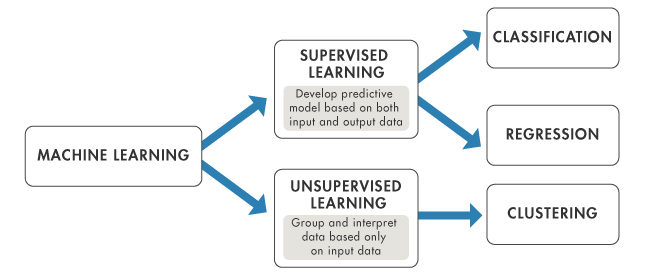
\includegraphics[width=350px]{chapters/03/images/machine-learning.png}
    \caption{\label{machine learning}, Machine Learning, \url{https://wiki.seg.org/images/1/10/Machine_learning_workflow_.png}}
\end{figure}

\paragraph{Apprentissage supervisé}

\paragraph{} Un algorithme d'apprentissage est dit \emph{supervisé} au sens où il lui est fourni des exemples de problèmes \emph{résolus} desquels
il doit effectuer son apprentissage, où \emph{un intermédiaire humain} à pris le temps \emph{d'étiquetter} un certain nombre de cas avec la bonne réponse.
L'apprentissage de l'algorithme s'effectue alors à partir du fait qu'il devient meilleur à l'exécution d'une même tâche donnée en se référant aux exemples
de ce qu'il est supposé accomplir. Et pour ce faire, cet algorithme d'apprentissage supervisé à besoin d'un outil particulier : \emph{un modèle}.

\paragraph{Qu'est-ce qu'un modèle ?} Comme nous l'avons vu précédemment, le Machine Learning intervient lorsque l'Homme devient \emph{incapable de modéliser un mapping},
c'est-à-dire lorsque nous ne pouvons deviner l'affectation qu'il doit y avoir entre des entrées données et les sorties possibles. Un modèle dans ce contexte se réfère 
exactement \emph{au mapping} : c'est un ensemble de règles que prend un problème en entrée et qui possède une réponse. Ce modèle peut être très simple (une règle seule)
tout comme il peut être arbitrairement complexe (combinaisons de jeux de règles complexes et inter-indépendants). On peut également dire qu'un modèle est la solution à un problème
\emph{en général}, en donnant les réponses à des \emph{instances de problèmes spécifiques}. Autrement dit, un modèle permet de répondre à des \emph{use-cases spécifiques} du
\emph{domaine d'un problème} \cite{MachineLearning3} : lorsqu'il lui est fourni un \emph{ensemble de valeurs numériques} représentant une instance de problème spécifique, il répondra
avec \emph{un ensemble de valeurs numériques} représentant la réponse à cette instance.

\paragraph{Comment l'entrainer ?} Il existe de nombreuses théories quant à la manière d'entraîner un modèle, aussi nous focaliserons-nous ici sur le \emph{procédé global}
permettant d'aboutir à un modèle entrainé. Au départ, l'algorithme commence avec un plan de modèle, assimiliable à un \emph{modèle vierge}, qui renvoie des solutions 
absolument incorrectes. Ce modèle à un nombre de \emph{paramétrages} qui déterminent les réponses fournies. Ce sont ces paramétrages que l'algorithme de machine learning va
modifier, tester, régler jusqu'à ce que le modèle \emph{fournisse des solutions plutôt précises} - la notion de \emph{plutôt} étant elle-même déterminée par la machine.
Pour ce faire, l'algorithme va \emph{considérer chaque exemple fourni} (par notre jeu de données, soigneusement préparé) et \emph{l'essayer sur le modèle}. Il compare ensuite
la réponse obtenue à la réponse correcte, et remodifie ses \emph{paramétrages} afin qu'il produise par la suite une réponse \emph{un peu meilleure} que celle qu'il a fournie.
Ce processus peut être répété plusieurs fois sur le même jeu de données, pour tenter d'améliorer \emph{la précision} de l'algorithme. Dans la plupart des cas, à l'instar d'AlphaGo
Zero \cite{AlphaGo2}, la courbe d'apprentissage s'apparente à une courbe logarithmique : plus l'apprentissage avance, plus il est compliqué d'améliorer l'algorithme en question.
Une fois l'apprentissage terminé, le modèle, qui à été entraîné sur un jeu de données particulier, doit en théorie être appliquable à \emph{toute instance de problème spécifique}.

\paragraph{Comment l'utiliser ?} L'apprentissage supervisé est utilisé principalement lorsque nous voulons qu'un ordinateur accomplisse une tâche pour laquelle nous avons un grand nombre
d'exemples avec une réponse associée, sans pour autant connaître les étapes pour parvenir à cette réponse. Ce type d'algorithmes est largement utilisé et nous avons déjà évoqué plusieurs
systèmes s'appuyant sur ces algorithmes, à l'exemple de :
\begin{itemize}
    \item La détection de spams - Permet de garder votre boîte de réception propre après avoir appris de nombreux exemples de spams
    \item La reconnaissance d'objets ou de comportement - A partir d'images ou de vidéos
    \item La reconnaissance de l'écriture - Aussi appelés OCR (Optical Character Recognition), ces logiciels permettent par exemple de reconnaître les adresses sur les
    enveloppes postales ou encore les signatures
    \item Biologie génétique - Reconnaître des séquences d'allèles
    \item Médecine préventive - Dépister à l'avance certaines maladies par l'étude de diagnostics médicaux
    \item La prédiction - Deviner une information à l'avance \cite{MachineLearning2}
\end{itemize}

\paragraph{Classification et Regression} Lorque nous pratiquons l'apprentissage supervisé, il faut choisir en amont entre deux catégories d'algorithmes : classification ou
regression. Leur différence peut s'illustrer de manière très simple par l'exemple suivant :

\begin{figure}[h]
    \centering
    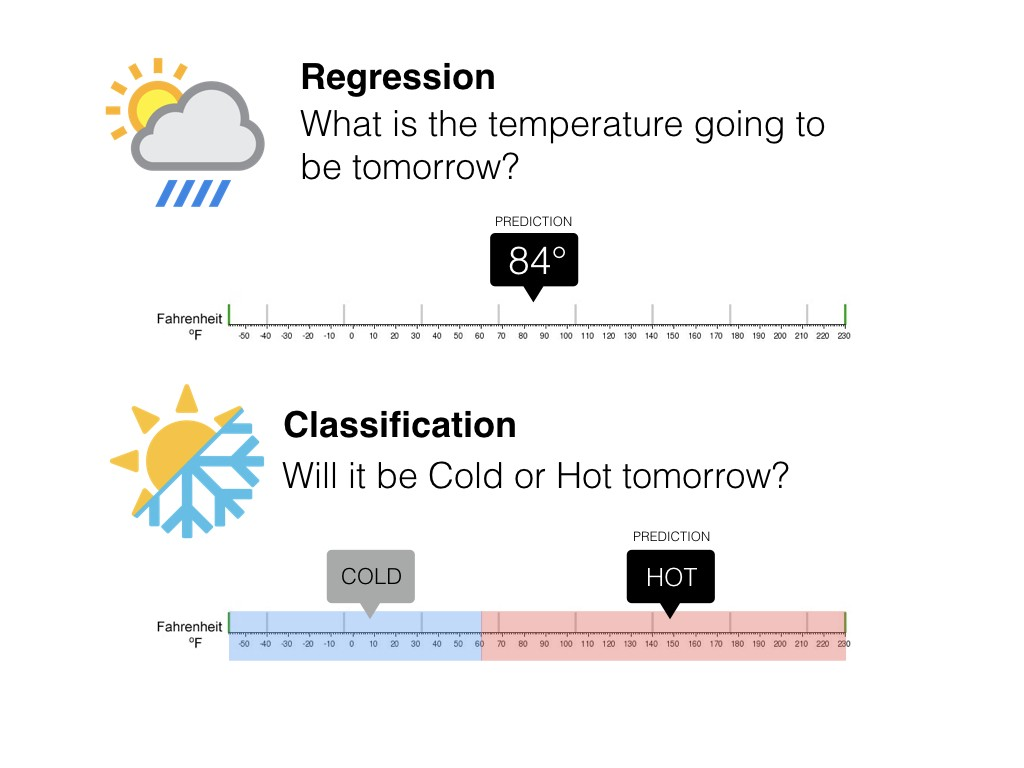
\includegraphics[width=300px]{chapters/03/images/classification-regression.jpg}
    \caption{\label{supervised learning}, \emph{Classification and Regression}, \cite{MachineLearning6}}
\end{figure}

\paragraph{} Un algorithme d'apprentissage supervisé par regression prédit une valeur \emph{continue}, c'est à dire la valeur \emph{précise} attendue pour une instance de problème donnée.
La réponse de cet algorithme n'est donc pas \emph{binaire} : c'est une valeur, un pourcentage, un indice, un indicateur. Plusieurs outils mathématiques, appartenant en particulier aux
domaines de la statistique et de l'analyse, permettent la mise en place de ces algorithmes \cite{MachineLearning3} : régression linéaire \cite{MachineLearning4}, régression polynomiale, régression pas à pas 
\cite{University1}, régression Ridge et LASSO \cite{University0}. De leur côté, les algorithmes d'apprentissage supervisé par classification permettent de prédire \emph{l'appartenance} de la
solution à un \emph{groupe} donné. Ce n'est pas une valeur qui est prédite : l'algorithme se contente de \emph{classer} les solutions en plusieurs catégories (d'où le terme de classification)
et, lorsqu'il lui est donné une nouvelle entrée, d'arriver à déterminer quelle catégorie est la plus appropriée pour cette entrée. On remarquera dans la pratique que les réseaux neuronaux
permettant de modéliser ces algorithmes sont \emph{pratiquement semblables}. En effet, les premières couches auront le rôle \emph{d'approcher} une solution existante, dans les deux cas en
s'appuyant sur l'ensemble des données fournies. Ce sont les dernières couches du réseau, les couches \emph{décisionnelles}, qui se chargeront de transformer l'information reçue en une décision
de type \emph{regression ou classification}. Le procédé reste donc globalement similaire.

\paragraph{} On remarquera que \emph{les accès} aux méthodes du Machine Learning sont encore restreints : ce domaine nécessite à la fois des connaissances conséquentes dans d'autres domaines 
à forte composante mathématique ainsi que des systèmes informatiques développés afin de \emph{stocker de large quantités de données} et \emph{d'effectuer efficacement des calculs} sur ces
dernières. De plus, il n'existe pas d'outil \emph{simple et libre} permettant d'appliquer les principes du ML sans apprentissage préalable. Le background nécessaire pour participer à la création 
et l'entrainement d'un modèle est riche, et l'utilisation de ces techniques est donc réservé à une \emph{population possédant un niveau de formation élevé}. Dans cette mesure, nous pouvons
questionner l'éthique d'utilisation des techniques du Machine Learning. Etant donné que ces techniques sont réservées à une partie de la population, et qu'elles lui permettent d'acquérir 
\emph{une connaissance plus précise du fonctionnement de l'ensemble de la population}, elles contribuent en un sens à \emph{accentuer les disparités entre les classes sociales}. Nous reviendrons
sur ce point important lorsque nous aborderons les usages et dérives associés à l'intelligence artificielle.

\paragraph{Apprentissage non supervisé, GANs}

\paragraph{} Lorsque nous parlons d'apprentissage non supervisé, on entend que les algorithmes n'ont au départ \emph{aucune
réponse} sur laquelle s'appuyer, et qu'ils doivent donc apprendre la structure des données par eux-même. Pour apprendre, il
est fourni à cet algorithme un \emph{très grand nombre} de données. Il essaie d'y discerner des groupes, des similarités ou
des déviations, ainsi que des \emph{patterns} (modèles) particuliers. Ces algorithmes sont en particulier utilisés afin de
discerner \emph{des groupes ou segments} dans les données, ou encore afin de construire des représentations visuelles de la
donnée.

\begin{figure}[h]
    \centering
    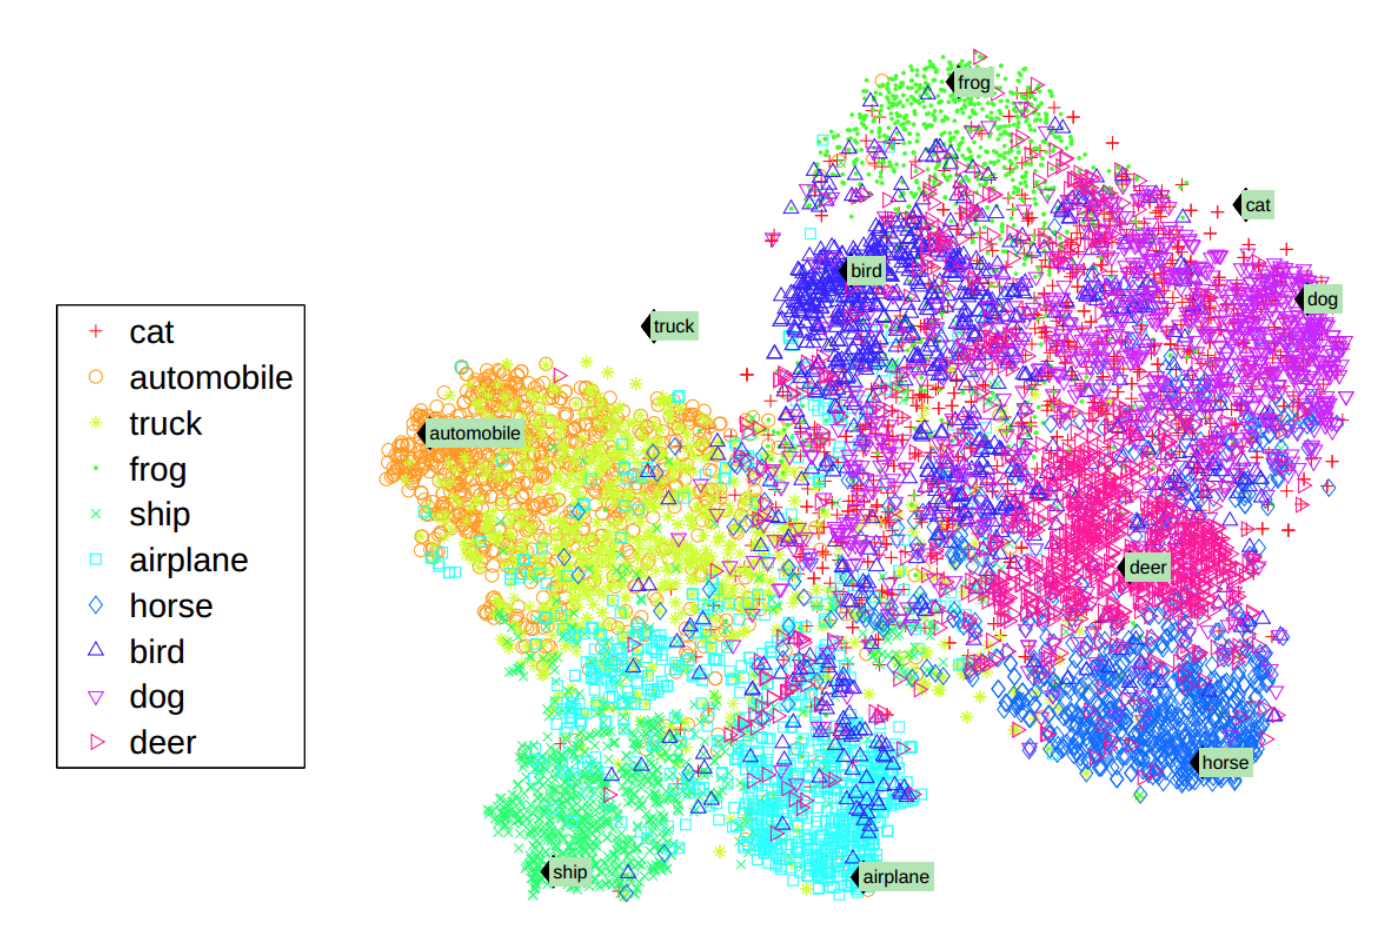
\includegraphics[width=300px]{chapters/03/images/clustering.png}
    \caption{\label{clustering} \emph{Group distinction by unsupervised learning}, \cite{MachineLearning0}}
\end{figure}

\paragraph{} Ces algorithmes apprennent en particulier à détecter les anomalies dans les groupes, ce qui permet par 
exemple de déterminer \emph{un comportement suspect} dans un lieu public. En sécurité informatique, sur internet, 
les algorithmes de machine learning peuvent détecter des éléments anormaux dans une source aussi riche que le trafic
d'un réseau. 

\paragraph{Generative Adversarial Networks} Selon Yann Le Cun, ils seraient une des inventions les plus pertinentes
des 10 dernières années dans le milieu du machine learning. Les Generative Adversarial Networks, simplifié par GAN,
consistent en deux types de modèles utilisés ensemble :

\begin{itemize}
    \item Un modèle \emph{discriminatif}, qui se charge d'apprendre à faire la différence entre une donnée \emph{authentique}
    et une donnée \emph{créée} par un modèle génératif.
    \item Un modèle \emph{génératif}, qui va essayer d'apprendre \emph{comment générer} une donnée de sorte à ce 
    qu'un modèle discriminatif \emph{n'arrive pas} à faire la différence avec une donnée authentique.
\end{itemize} 

\paragraph{} Bien que ces deux modèles soient utiles séparemment, ils le sont encore davantage couplés, appliqué à des cas
du monde réel, ou \emph{l'étiquettage de la donnée est souvent cher} \cite{MachineLearning5}. On peut assimiler leur travail
à celui \emph{d'un faussaire et d'un policier} (génératif et discriminatif). C'est un fait qui nous interpelle et nous fait
comprendre l'importance que leur apportent les chercheurs : en prenant à la fois le rôle de \emph{créateur de faux} et de
\emph{distinguer le vrai du faux}, les GANs permettent de saisir le \emph{comportement sous-jacent} d'un système, qu'il serait
impossible d'approcher pour un humain. Cela ouvre de nouvelles perspectives pour la compréhension de problèmes complexes de
domaines aussi divers que les mathématiques, l'informatique, la finance, la médecine.. ou des problèmes tels que celui d'Ada !

\paragraph{AlphaGo, AlphaGo Zero}

\paragraph{} Courant 2016 et 2017, une annonce à fait grand bruit dans le milieu de l'intelligence artificielle
suite à un événement particulier : une IA avait enfin réussi à battre un des meilleurs joueurs professionnels de Go
au monde, Lee Sedol. Nous allons revenir sur l'évolution du projet AlphaGo de \emph{Google DeepMind} ces deux dernières
années et essayer de comprendre pourquoi cela marque une des avancées les plus importantes des cinq dernières années
dans le milieu de l'IA et du \emph{Deep Learning} en particulier.

\paragraph{Jeu de Go, complexité infinie ?} Le jeu de Go est né en Chine il y a plus de 2500 ans. C'est un jeu de stratégie
se déroulant sur un plateau, le \emph{Goban}, sur lequel est tracé un quadrillage de 19 lignes sur 19 colonnes. Chaque joueur
pose, chacun son tour, une pierre de sa couleur (noire ou blanche) afin de tenter de posséder plus de \emph{territoire} que
son adversaire. Allégorie de l'Univers dans le monde oriental, le go se distingue en effet de tous les autres jeux de stratégie
par son immense complexité combinatoire. Le nombre de positions légales est estimé à \begin{math}10^{170}\end{math} sur un goban
de 19x19 contre \begin{math}10^{40}\end{math} aux échecs, et l'arbre de jeu couvre à lui seul plus de \begin{math}10^{600}\end{math}
parties plausibles contre environ \begin{math}10^{120}\end{math} aux échecs. A titre indicatif, le nombre d'atomes dans l'Univers est
de l'ordre de \begin{math}10^{79}\end{math}, la complexité du jeu de go est donc \emph{bien trop importante} pour essayer de l'approcher
avec des algorithmes classiques, ce qui explique qu'aucune IA d'un niveau réellement acceptable (c'est-à-dire proche de celui de
professionnel) n'ait été conçue avant AlphaGo.

\paragraph{AlphaGo, application réussie du Machine Learning}

\paragraph{} Quels sont les secrets d'AlphaGo ? Afin de calculer la valeur 
d'une partie \emph{dans un état donné}, AlphaGo utilise le MCTS ou Monte Carlo Tree Search. Cet algorithme permet d'analyser
quels sont les coups les plus pertinents à partir de l'étude de l'expansion \emph{d'une arborescence} \cite{Heuristics0}.
Néanmoins l'utilisation du MCTS à elle seule ne permet d'atteindre qu'un niveau semi-professionnel, c'est pourquoi il a été
utilisé un système de Deep Learning mettant en jeu des réseaux de neurones avec deux responsabilités distinctes : le
\emph{Policy Network} (ou réseau stratégique) et le \emph{Value Network} (ou réseau de valorisation) \cite{AlphaGo0}.

\paragraph{Réseau stratégique} L'entrainement de ce réseau à nécessité deux étapes de machine learning. Une première partie à 
consisté en l'apprentissage supervisé du réseau, auquel à été fourni 30 millions de positions à partir des parties recensées sur 
le KGS Go Server (serveur mondial de jeu de go). Suite à cet entraînement le réseau à été capable de prédire les coups joués par 
des professionnels avec une précision de 57\%. Une deuxième étape à été consacrée à l'apprentissage par renforcement, afin d'aider
à la prédiction des meilleurs coups possibles. Suite à un entrainement de plus d'un million de parties contre lui-mêmme, le réseau
renforcé à été capable de battre le réseau non renforcé dans plus de 80\% des cas. A ce stage le réseau possède encore un niveau
d'amateur - environ 3e dan sur le KGS Go Server. \cite{AlphaGo1}

\paragraph{Réseau de valorisation} L'objectif du réseau de valorisation est de se focaliser sur l'évaluation de la position à un
instant donné. L'entrainement précédent ayant conduit à de \emph{l'overfitting} (le réseau tente de mémoriser les issues des parties
plutôt que \emph{généraliser des positions nouvelles}), un nouvel entraînement à été généré à partir des parties jouées contre
lui-même, soit plus de 30 millions de positions provenant d'autant de parties.

\paragraph{Les Résultats} En 2015, AlphaGo est la première machine à remporter des parties contre un professionnel, Fan HUI (2e dan professionnel
français). Il est ensuite le gagnant de parties importantes : contre Lee Sedol (9e dan coréen), considéré comme un des meilleurs professionnels
au monde, puis contre Ke Jie (9e dan chinois) qui est alors classé 1er au rang mondial. Il gagne aussi dans 99.8\% des cas contre
les meilleurs programmes, comme Crazy Stone, Pachi ou Zen. De plus, la version distribuée d'AlphaGo gagne 77\% de ses parties
contre la version non distribuée, ce qui signifie qu'AlphaGo est aussi bien \emph{performant que scalable}.

\paragraph{AlphaGo Zero, la révolution}

\paragraph{} Contrairement à AlphaGo qui à été entrainé au départ par l'étude de parties de professionnels, la version Zero d'AlphaGo saute
cette étape et apprend en jouant directement contre elle-même. Une nouvelle forme \cite{AlphaGo2} d'apprentissage par renforcement lui permet
d'être son propre professeur. Au départ, le réseau neural ne connait rien du jeu de go si ce n'est les règles, et joue donc des coups aléatoires.
Pendant la partie, le réseau neural se met à jour afin d'améliorer son système de prédiction. AlphaGo Zero joue ainsi contre sa nouvelle version,
et ainsi de suite jusqu'à ce qu'il gagne réellement en niveau et que le réseau s'optimise. Cette technique est bien plus puissante que les anciennes
versions d'AlphaGo car elle n'est plus contrainte par \emph{les limites de la connaissance humaine}. 

\paragraph{} La version Zero se démarque aussi des précédentes par trois points :

\begin{itemize}
    \item Elle n'utilise \emph{que les pierres noires et blanches comme input}
    \item Elle n'utilise \emph{qu'un réseau de neurones} plutôt que deux. La version Zero combine ici le réseau stratégique et le réseau de valorisation.
    \item Elle n'utilise plus le principe \emph{de rollouts}, qui lui permettait de prédire plus rapidement mais moins précisément a partir de l'étude de parties d'autre programmes. 
\end{itemize}

\paragraph{} Après seulement trois jours d'auto-apprentissage, AlphaGo Zero arrivait à battre la version la plus aboutie d'AlphaGo à raison de 100 parties à 0,
et devenait alors la meilleure IA jamais conçue pour le jeu de go. Enfin, la version Zero possède aussi une consommation en énergie bien plus faible.

\begin{figure}[h]
    \centering
    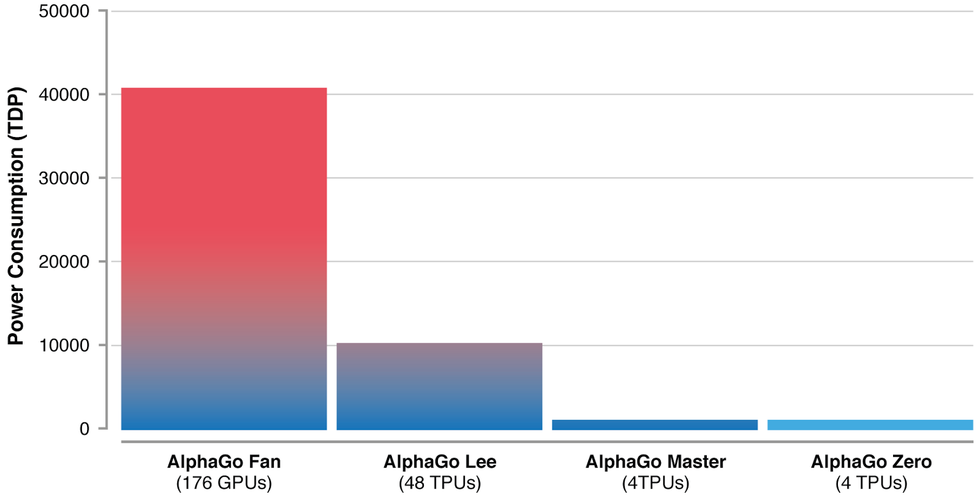
\includegraphics[width=300px]{chapters/03/images/alphago-consumption.png}
    \caption{\label{comparatif}, \emph{Power consumption for each AlphaGo version}, \cite{AlphaGo2}}
\end{figure}

\paragraph{La clé de la réussite d'AlphaGo Zero} Ce dernier se démarque également par son architecture un peu particulière,
aussi qualifiée de \guillemotleft monstre à deux têtes\guillemotright. \cite{AlphaGo3} En effet, après les 20 premières
couches ou \emph{blocks}, se trouvent deux \emph{têtes} : une qui va faire une prévision sur le joueur qui est actuellement
en train de gagner, une qui calcule la probabilité de jouer tel ou tel coup. C'est un fait inhabituel en comparaison à tous
les systèmes dont il à été question jusqu'ici, qui ne restituaient qu'\emph{une sortie unique} (comme une image, l'appartenance
à un groupe, une valeur précise).

\paragraph{} La question se pose alors du \emph{fonctionnement} d'un tel système. Et il est en fait \emph{identique}
à ce que nous avons vu jusqu'alors : lorsque la première \emph{tête} fait une prédiction, cela met à jour le modèle
du \emph{corps}; et de la même manière pour la seconde tête. De cette façon, l'évolution à chaque tour est plus importante
puisque ce ne sont plus une mais deux mise à jour des couches neuronales qui sont effectuées. Cela permet bien évidemment
un renforcement plus important et plus rapide de notre système, mais cela ouvre également à la création de nouveaux systèmes :
les réseaux neuronaux \emph{multi-têtes}.

\paragraph{De la puissance multi-domaines des sorties multiples}

\paragraph{Applications aux données humaines}

